
\begin{wrapfigure}{r}{0.25\textwidth}
  \begin{center}
    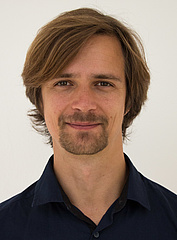
\includegraphics[width=0.2\textwidth]{foto}
  \end{center}
\end{wrapfigure}


{\large{\bf{Dipl.-Phys.~Dr.rer.nat.~Matthias Schl\"ogl}}} \\[1ex]
    Rabnitzweg 18B/3 \\
    8063 Eggersdorf, Austria \\
    matthias.schloegl@gmx.de\\
    +436804029054 \\
   \url{http://mschloegl.github.io}

% Institute of Medical Engineering,  \\
% Graz University of Technology,  Stremayrgasse 16/III, A-8010 Graz
%{
  %\setlength{\topsep}{0pt}%
  %\setlength{\partopsep}{0pt}%
%  \begin{tabbing}
%
%    E-mail: \quad \= m.schoegl@solgenium.com\\
%    %Web: \> \url{http://www.tugraz.at/institute/imt/people/schloegl/} 
%  \end{tabbing}
% }  
%%%%%%%%%%%%%%%%%%%%%%%%%%%%%%%%%%%%%%%%%%%%%%%%%%%%%%%%%%%%%%%%%%%%%%%

\vspace{0.8cm}
{\bf Personal Data}
\begin{tabbing}
\vspace{0.2cm}
Date and place of birth: \quad \=\kill
Date and place of birth: \>  2.5.1985, Nabburg, Germany\\
Citizenship: \> German\\
married, two daughters
\end{tabbing}


%%%%%%%%%%%%%%%%%%%%%%%%%%%%%%%%%%%%%%%%%%%%%%%%%%%%%%%%%%%%%%%%%%%%%%%

%\vspace{0,6cm}
%{\bf Main research areas}
%\vspace{0,2cm}

%\begin{compactitem}
%\item 
%  Accelerated (dynamic) MR Image reconstruction with variational constraints 
%\item 
%(Dynamic) MR Image reconstruction with integrated artifact correction and parameter estimation
%\end{compactitem}



%%%%%%%%%%%%%%%%%%%%%%%%%%%%%%%%%%%%%%%%%%%%%%%%%%%%%%%%%%%%%%%%%%%%%%%

\vspace{0.7cm}
{\bf Education\\}
%\vspace{0.2cm}
\noindent\rule{\textwidth}{0.5pt}
\begin{tabbing}  
	2012 - 2018 \quad \= \emph{\textbf{Dr.rer.nat. Computer Science and Biomedical Engineering}} \\
  	\> Graz University of Technology, Institute of Medical Engineering, Graz, Austria  \\ %(Grade: 1.14)\\
  	\> PhD-Thesis: \emph{Spatio-temporal image reconstruction} \\
  	\> \emph{for accelerating dynamic MRI applications using variational priors.} \\

	2006 - 2011 \quad \= \emph{\textbf{Physics (Dipl.-Phys.)}} \\ %(Grade: 1.14)\\
  	\> University of Regensburg, Regensburg, Germany \\
	\> and Universidad de Granada, Granada, Spain. \\
	\> Diploma-Thesis: \emph{Bayesian segmentation of MR images using the $\alpha$-stable distribution}\\
	\> \emph{Application to dementia disease detection}. \\
  
	2005 - 2006 \quad \= \emph{\textbf{Microsystems Engineering}} \\
	\> University of Applied Sciences, Regensburg, Germany \\
 
	2004 \quad \quad \quad \quad \= \emph{\textbf{Abitur}}\\  
	\> Johann-Andreas-Schmeller Gymnasium, Nabburg, Germany %(Grade: 2.3) \\
 
\end{tabbing}
\bigskip


%%%%%%%%%%%%%%%%%%%%%%%%%%%%%%%%%%%%%%%%%%%%%%%%%%%%%%%%%%%%%%%%%%%%%%%%%%
\vspace{0.7cm}
{\bf Professional Appointments}\\
\noindent\rule{\textwidth}{0.5pt}
%\vspace{0.2cm}
\begin{tabbing} 
since 01/2019 \quad \quad \quad \= \emph{\textbf{Data Scientist}}\\
 \> Solgenium OG, Linz, Austria \\

03/2012 - 12/2018 \quad  \= \emph{\textbf{Research Assistant}}\\
  \> Institute of Medical Engineering\\
  \> Graz University of Technology, Graz, Austria \\
\end{tabbing}
\bigskip

%%%%%%%%%%%%%%%%%%%%%%%%%%%%%%%%%%%%%%%%%%%%%%%%%%%%%%%%%%%%%%%%%%%%%%%%%%
{\bf Academic Awards}\\
\noindent\rule{\textwidth}{0.5pt}
%\vspace{0.2cm}
\begin{tabbing} 
2015 \quad \= International Society for Magnetic Resonance in Medicine: \\
  \> Summa Cum Laude Award. \\
2013 \quad \= $2^{{nd}}$ place ISMRM reconstrution challenge 2013 (\url{challenge.ismrm.org/node/67}) \\
\end{tabbing}


%\vspace{0,7cm}
%{\bf International Experience}
%\vspace{0,2cm}
%\begin{tabbing} 
%2005 - 2006 \quad \= Travel \& Workprogram, Australia and New-Zealand \\
%2009 - 2010 \>  Erasmus program, Granada, Spain
%\end{tabbing}
%\bigskip

%%%%%%%%%%%%%%%%%%%%%%%%%%%%%%%%%%%%%%%%%%%%%%%%%%%%%%%%%%%%%%%%%%%%%%%%%%
\vspace{0.7cm}
{\bf Languages}\\
\noindent\rule{\textwidth}{0.5pt}
%\vspace{0.2cm}
\begin{tabbing} 
	\textbf{German} \quad \= First language \\
	\textbf{English} \>  Business fluent \\
	\textbf{Spanish} \>  Fluent \\
	\textbf{French} \> Basic
\end{tabbing}
\bigskip

%%%%%%%%%%%%%%%%%%%%%%%%%%%%%%%%%%%%%%%%%%%%%%%%%%%%%%%%%%%%%%%%%%%%%%%%%%
\vspace{0.7cm}
{\bf Skills}\\
\noindent\rule{\textwidth}{0.5pt}
%\vspace{0.2cm
\begin{tabbing}
\textbf{Research interests} \quad \quad \quad \quad \quad \quad \= Magnetic resonance imaging, medical imaging\\ 
	\> inverse problems, optimization, machine learning\\
	\> bayesian data analysis, operational research\\
\textbf{Programming languages} \> Python, R, STAN, bash, SQL, C/C++, CUDA, scala\\
\textbf{Specific libraries} \> tensorflow, tensorflow probability\\
\textbf{DevOps} \> git, gitlab CI/CD, docker, google cloud platform\\
\textbf{Other} \> latex, microsoft office\\
\end{tabbing}
\bigskip

%%%%%%%%%%%%%%%%%%%%%%%%%%%%%%%%%%%%%%%%%%%%%%%%%%%%%%%%%%%%%%%%%%%%%%%%%%
%\vspace{0,4cm}
%{\bf Invited Presentations}
%\begin{tabbing}
%2013 \quad \= RTaustria Kongress Salzburg: \\
%\> Bildrekonstruktion f\"ur beschleunigte MR Bildgebung:   Mathematik trifft Radiologie\\
%\end{tabbing}



%%%%%%%%%%%%%%%%%%%%%%%%%%%%%%%%%%%%%%%%%%%%%%%%%%%%%%%%%%%%%%%%%%%%%%%
\vspace{0.7cm}
{\bf Contributed Research Proposals}\\
\noindent\rule{\textwidth}{0.5pt}
%\vspace{0.2cm}
\begin{tabbing}
2020 \= \textbf{FFG Covid-19 mergency call}\\
  \> Covid-19 optimization of resource allocation. \\ 
2017  \= \textbf{FWF and CDP Project PIR 27} \\
  \> Mathematical methods for motion aware medical imaging. \\ 
2016  \= \textbf{FWF SFB F32-N18} \\ 
  \> Mathematical optimization and applications in biomedical sciences. \\ 
\end{tabbing}
\bigskip

%%%%%%%%%%%%%%%%%%%%%%%%%%%%%%%%%%%%%%%%%%%%%%%%%%%%%%%%%%%%%%%%%%%%%%%
\vspace{0.7cm}
{\bf Talks}\\
\noindent\rule{\textwidth}{0.5pt}
%\vspace{0.2cm}
\begin{tabbing}
    2016 \=  Workshop on Imaging with Modulated/Incomplete data, Graz, Austria. \\ 
	 \> ICTGV reconstruction for accelerated Non-Cartesian DCE and quantitative MRI. \\
    2016 \> ESMRMB Annual Meeting, Vienna, Austria. \\
	 \> ICTGV Reconstruction of DCE golden angle radial VIBE data. \\
    2016 \> ISMRM Workshop on Data Sampling and Image Reconstruction, Sedona, USA \\
	 \> Accelerated Variational Dynamic MRI Reconstruction (AVIONIC) \\  
    2015 \> ISMRM Annual Meeting, Toronto, Canada. \\
	 \> ICTGV Regularization for Highly Accelerated Dynamic MRI.  
\end{tabbing}
\bigskip

\newpage
%%%%%%%%%%%%%%%%%%%%%%%%%%%%%%%%%%%%%%%%%%%%%%%%%%%%%%%%%%%%%%%%%%%%%%%
\vspace{0.7cm}
{\bf Invited Talks}\\
\noindent\rule{\textwidth}{0.5pt}
%\vspace{0.2cm}
\begin{tabbing}
     2018 \= University of Technology Brno, Brno, Czech republic.\\
	  \> ICTGV reconstruction for dynamic MR applications. \\
    2013 \>  RT Austria Kongress, Salzburg, Austria. \\
	 \> Bildrekonstruktion f\"ur beschleunigte MR Bildgebung: Mathematik trifft Radiologie
\end{tabbing}
\bigskip


%%%%%%%%%%%%%%%%%%%%%%%%%%%%%%%%%%%%%%%%%%%%%%%%%%%%%%%%%%%%%%%%%%%%%%%
\vspace{0.7cm}
{\bf Training}\\
\noindent\rule{\textwidth}{0.5pt}
%\vspace{0.2cm}
\begin{tabbing}
2019 \= STAN Con, Cambridge, UK. \\
2017 \> ESMRMB Workshop on Non-Cartesian MRI, W\"urzburg, Germany. \\
2016 \> ISMRM Workshop on Data Sampling and Image Reconstruction, Sedona, USA.\\
2014 \> ESMRMB Workshop on Compressed Sensing, Freiburg, Germany.\\
2013 \> ESMRMB Workshop on Parallel Imaging, W\"urzburg, Germany.
\end{tabbing}
\bigskip


%%%%%%%%%%%%%%%%%%%%%%%%%%%%%%%%%%%%%%%%%%%%%%%%%%%%%%%%%%%%%%%%%%%%%%%
\vspace{0.7cm}
{\bf Software}\\
\noindent\rule{\textwidth}{0.5pt}
%\vspace{0.2cm}
\begin{tabbing}
	\textbf{AVIONIC} \=  Accelerated Variational dynamic MRI reconstruction. \\
	\> \url{http://github.com/imttugraz/avionic}
\end{tabbing}
\bigskip

%%%%%%%%%%%%%%%%%%%%%%%%%%%%%%%%%%%%%%%%%%%%%%%%%%%%%%%%%%%%%%%%%%%%%%%
\vspace{0.7cm}
{\bf Teaching}\\
\noindent\rule{\textwidth}{0.5pt}
%\vspace{0.2cm}
\begin{tabbing}
2013 - 2017 \= Fundamentals of Biomedical Engineering, laboratory (717.300, Pacemaker, Blood Pressure).\\
2013 - 2017 \> Imaging laboratory (717.340, MRI Reconstruction).\\
2013 - 2015 \> Inverse Problems in Medical Imaging, practical course (717.324).
\end{tabbing}
\bigskip

